% -*- fill-column: 110 -*-
\documentclass[12pt]{article}
\usepackage[margin=1in]{geometry}
\usepackage{hyperref}
\usepackage{graphicx}
\usepackage{amsmath}
\usepackage{amsfonts}
\usepackage{amssymb}
\usepackage{amsthm}
\usepackage[margin=1in]{geometry}
% \usepackage{apacite}
\usepackage{color}
%\usepackage{sagetex}
\usepackage{fancyhdr}
\usepackage{setspace}
\pagestyle{fancy}
\lhead{\footnotesize Outline for IDS499 final project}
\rhead{\footnotesize October 12 2013 -- IDS499 -- Shae Erisson}

\author{Shae Matijs Erisson\\Interdisciplinary Studies Department\\University of North Alabama}
\title{Statistical Learning for User-Specific Webpage Recommendations}
\begin{document}
\date{October 12 2013}
\maketitle{}
\pagebreak{}
%\section*{Statistical Learning for User-Specific Webpage Recommendations}

\begin{abstract}
  This paper and its associated software will explore the use of statistical learning to find previously
  unknown webpages of interest to the user of the software.

  We focus on the use of support vector machines to do supervised learning that results in efficient
  categorization of web pages into interesting or uninteresting.

  We also present a prototype web-based tool that allows the user to train their own nonlinear statistical
  classifier to find web pages specific to a particular subject of interest.
\end{abstract}
\pagebreak{}
\section{Introduction}
Can statistical classifiers be used to expand rather than filter knowledge?

Much time is spent trying to find relevant web sites when doing research for any number of tasks. While those
helpful websites exist for almost any subject, it can be difficult to find which website is best for a
particular topic.

While searching Google can be fun, sometimes too much time is spent trying to find relevant information, or
irrelevant search results become distrating from the actual

Up to now statistical classifiers such as Bayesian statistics have primarily been used to automatically
categorize items based on a user's feedback. In fact, this is how most spam filters function. Since each
person will consider different messages to be useful content, and so each person must give their own feedback
to the filter.

Services such as Netflix and Amazon use similar software to suggest movies or books according to which movies
or books the user has already enjoyed.

The research problem we address here is whether this can be generalized to recommending webpages to the user
according to which webpages they've found relevant in the past.
\section{Justification for the Study}
Statistical learning has been used to filter spam for decades. In that specific case, the filtering works by
increasing or decreasing the score of a particular message by summing the score of each word in the contents.
These statistics are trained for each user, so the word mortgage might have a positive score for a bank
employee, where mortgage would have a negative score for most people.

This research project proposes to use support vector machines to find new results rather than filter out
existing content. The project consists of both prototype software and a report describing the results.

% The software will watch the user browsing the web and uses that input to build Bayesian statistics for later
% searching for new documents of interest.
\section{Statistical Classifiers}
% This section will give an overview of statistical classifiers. 

The goal of a classifier is to sort inputs into different categories based on features of those inputs. The
most familiar examples would be book recommendations from Amazon and movie recommendations from Netflix. Those
recommendations are done with software that has determined important features of all the books and movies
available, and has some way to figure out which books or movies are similar to which other books or
movies. \cite{michie1994machine}



Statistical classifiers are divided into two major types, linear classifiers and non-linear classifiers.
\subsection{Linear Classifiers}
%This section will describe the simplest instance of linear statistical classifiers, Naive Bayesian
Linear classifiers are called linear because, given a set of points drawn in a two dimensional space, the
classifier finds a line that divides the space into two halves where one side of the line is one category, and
the other side of the line is the other.\\
% center this? XXX
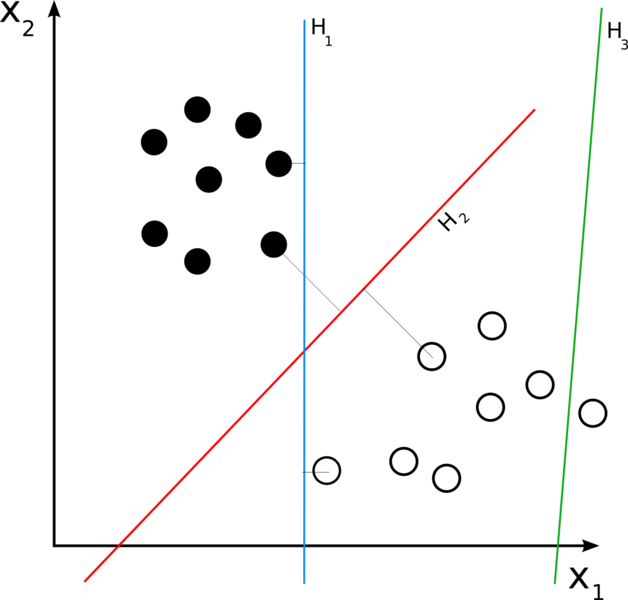
\includegraphics[scale=.4,natwidth=628,natheight=600]{svm_separating_hyperplanes.png}\\

The most popular linear classifier is the Naive Bayesian classifier. \cite{kononenko1991semi}
We will describe the use of a Naive Bayesian Classifier for classification of email into so called ham and
spam messages. Spam is common jargon used to describe unwanted email, most often containing advertising or
some other attempt to extract money from the recipient of that email. Ham is a lesser known word that
describes a message that has actual content that the user wishes to receive.

In summary, each word in an email has a particular positive or negative value associated with it from earlier
training. These values are added together, and the resulting sum is compared against user-specified
thresholds. If the value is greater than the ham threshold, the message is considered content and displayed to
the user. If the value is less than the spam threshold, the message is considered spam and is sent to a spam
folder on the user's email system.

Obviously when a user is first added to an email system, they cannot have given any input to the system, and
thus the training values are empty, and all messages are considered ham. The most popular user interface
approach is to add a button that allows a user to classify any message as spam. When that happens for the very
first time, the software changes the values of all the words in the message to a negative value. After that
very first input of training data, any message that contains words that were found in the spam message will be
marked as spam. 

On the other side of the problem, the user has the ability to view the spam folder and mark any of those
messages as ham. At that point, it is almost certain that some words will have appeared in both the ham and
spam categories. 

This leads to an interesting problem. How can we determine what new value should be given to a word that has
appeared once in a ham message, once in a spam message, and then user input tells us that the word has
appeared once again in a spam message?

The Reverend Thomas Bayes was both a Presbyterian minister and a mathematician, and his research into what was
then called inverse probability became Bayes theorem. The idea of inverse probability started out with the
question: given an urn containing a certain number of black and white balls, what is the probability of
drawing one particular color of ball? Then, once a ball of a black or white ball has been removed, what is the
new probability of drawing out a ball of a particular color? This sort of question applies directly to the
spam classification problem, since it requires that we calculate the probability that a word will be in a spam
message based on a combination of the number of times it has been found in spam and ham messages.

% http://en.wikipedia.org/wiki/Bayes'_theorem#Events
$$P(A|B)= \dfrac{P(B|A)P(A)}{P(B)}$$

% We shall use $P(S)$ to denote the probability that a word will be found in a spam message, and $P(H)$ to
% denote the probability that a word will be found in a ham message. $P(B|A)$, or
This form of Bayes' Theorem requires that we know the prior probability that a word will be in a spam
message, and given a fixed event such as a word being marked spam, will give us the new probability of that
word being found in a spam message. This new probability is called the posterior probability. 

In the case where a word has appeared once as ham and once as spam, the prior probability is .5, or 50\%. 
$$P(W) = .5$$
The probability of a message being spam is denoted as $P(S)$, and the probability of a message being ham is
$P(H)$. Both of these are calculated putting all the probability values of all the words in a message into
Bayes' Theorem.

In probability, the likelihood of one event $B$ happening after an event $A$ has happened is denoted as
$P(B|A)$. We will be using this to figure out the probability that a message is spam once we know the chance
that a particular word is found in a spam message, denoted as $P(M|W)$.

We calculate the total probability that a message is spam by combining all of the individual probabilities.
In the equation below, $p_{1}$ is the probability that the first word is spam, $p_{2}$ is the probability that
the second word is spam, and so on until word $n$.
$$p=\dfrac{p_{1}p_{2} ... p_{n}}{p_{1}p_{2} ... p_{n} + (1-p_{1})(1-p_{2}) ... (1-p_{n})}$$

Where $p$ is the overall probability that a message is spam, given $p_{1}$, the probability that the first
word will be found in a spam message, and $p_{2}$, the probability that the second word will be found in a
spam message, and so on up to the last word in the message.
% http://en.wikipedia.org/wiki/Bayesian_spam_filtering#Computing_the_probability_that_a_message_containing_a_given_word_is_spam

% Once the word has been marked a second time as spam, we can fill in the values and calculate the new
% probability. Since this word has been marked as spam, the probability of this event is 100\% and $P(W)$ is 1.
% $$P(M|W) = \dfrac{P(M|W)P(W)}{1}$$
% Thus, the new probability of this particular word being found in a spam message is

\subsection{Non-Linear Classifiers}
Non-linear classifiers are described as such because they are able to separate points into multiple regions
rather than only being able to divide a cloud of points into two parts. This is useful when multiple the
inputs need to be divided into multiple categories. 
\subsection{Others}
% XXX put something about the others here?
% This section will cover the range of other statistical classifiers in less detail.
The first linear classifiers were described in 1936. \cite{fisher1936use} As mentioned earlier, they could
only find a single line across a plane to divide many points into two groups.  In 1962, the first research on
neural networks was published. Each neuron in a neural network was a separate linear classifier, giving them
the ability to combine multiple separate group divisions into a piece wise linear separation. In the mid 1980s
the back propagation algorithm was discovered that allowed errors in classification to be propagated backwards
through the network to change the value for each separate node in the network. \cite{cortes1995support}
\subsection{Support Vector Machines}
% http://www.youtube.com/watch?v=qyyJKd-zXRE andrew ng's video from the stanford course on machine learning
Bayesian classifiers are easy to understand both from the mathematical and implementation viewpoints, but are
less effective than non-linear classifiers. Non-linear classifiers such as neural networks are effective, but
do not produce knowledge that can be used outside of the neural network.  Support vector machines have the
great benefit that they are effective for two or many more categories, they are mathematically simple, and the
result of their training can be extracted and used for other purposes. \cite{hearst1998support} In addition,
support vector machines look for the largest margins between groupings of points, and thus automatically
produce classifiers that can be applied to new inputs as well as determining what features are unique to each
grouping. Part of the improvement found with support vector machines comes from their use of linear
classifiers after a non-linear remapping of the data. \cite{cortes1995support}

While earlier classifiers have concentrated on the contributing values for each point of data, the support
vector machine instead searches for the most widely separated values, as those will most often denote a group
of data points separate from other groups. This also requires far less computation than other algorithms.

Support vector machines can be equivalent to machine learning done with several other types of classifiers
such as polynomial classifiers, radial basis functions, and neural networks. \cite{hearst1998support}

% XXX lots more content could go here

\section{Common uses of Statistical Classifiers}
\subsection{Spam Filters}
Naive Bayesian spam filtering has had much been the subject of many research papers. It is perhaps
unsurprising that this linear classifier gives decent but not spectacular performance.  Bayesian spam filters
have been found to require continuous training in order to achieve good results, but have also found to be
imperfect even after thorough training on large collections of messages. Thus Bayesian spam filters are only
sufficient when backed up with other approaches.  \cite{androutsopoulos2000evaluation}
\subsection{Natural Language Guessing}
% This will describe how statistical classifiers are used in guessing the natural language used in a document.
If you've navigated your web browser to a web page written in a language other than your native language,
you've probably seen a small popup offer to translate from the language of the web page into your native
language. But how can computers discover the language of the document without asking the user?

Originally, software looked for characters or words that are unique to a particular language, but effective
language guessing software now looks for particular sequences of letters called n-grams. An n-gram is a
contiguous string of characters of length n. This works well on short snippets of text that may not exhibit
any words or characters unique to the language used, and is fast and easy to implement. This also gives this
approach a tolerance to errors in spelling or grammar. Unsurprisingly, this approach cannot differentiate
between very similar languages such as American English and British English. \cite{martins2005language}
\subsection{Sentiment Classification}
While most of machine learning focuses on categorization by topic, there are other interesting uses for these
algorithms.  Sentiment classification is used to attempt to extract the emotional content for a particular
piece of text. This has been used for many diverse purposes, from attempting to predict the outcome of an
election to attempting to predict the relative market share of different mobile devices.

This kind of classification is especially interesting to web sites that aggregate information from other
websites. One good example is the movie reviews from the website \url{rottentomatoes.com}, which attempts to
give an average rating to a movie by combining many reviews written by other people. \cite{pang2002thumbs}

While many features of documents can be easily extracted, emotional content is often subtle. A sentence as
simple as ``How could you think that?'' has no explicitly emotional words, but is obviously a negative
statement towards the previous statement. The most common approach to extracting emotional content has been to
first find words with explicit positive or negative content, and then find which words are most often
associated with those words. For example ``good'' or ``great'' may often be associated with positive
sentiments, but ``spectacular'' could just as easily be associated with ``failure'' or ``flop'' as
``success''.

Unsurprisingly, the Naive Bayes model is good, but not spectacular. The maximum entropy approach has better
results, but support vector machines do a better job than either of the two earlier algorithms. This supports
the choice of this project to use support vector machines for the prototype.
\subsection{Malware Detection}
Most virus scanner are only able to detect a computer virus or other malware once it has been discovered and
dissected by a human. At that point the features unique to that virus are then added to the virus scanner
database.  This process would be much simplified if computers were able to recognize unknown viruses either by
behavior or by examining a program before execution.

Existing research has used an n-gram approach similar to the language guessing approach described
earlier. While this is effective, most malware is transmitted in a compressed format. Unsurprisingly, guessing
the safety of an executable inside a zip file is just as difficult as guessing the language of a text file
inside a zip file.  

More recent systems have added the ability to recognize compressed files and decompress them before examining
them for malicious intent, and have reported success rates up to 87.3\%. \cite{perdisci2008mcboost}
\subsection{Movie and Book Recommendations}
This will describe how statistical classifiers are used to recommend movies \cite{basu1998recommendation} and
books \cite{linden2003amazon} based on the movies or books previously enjoyed by a user.

Amazon.com has an unusual problem in that they have a very large number of products, and a varying amount of
data for each user. New customers will have a very few purchases on their account, while long time customers
could have many thousands of purchases. How can large amounts of both user and product information be
processed, and yet recommendations returned in a very short amount of time?

One common approach is called collaborative filtering, where the purchases of the logged-in user are searched
to find other people who have bought those same items, and the other people's purchases are searched to find
items that the logged-in user has not yet purchased. The idea here is that people make similar purchases, and
once buying one item, they may be interested in items that other people purchased along with that item.
Collaborative filtering can lead to wildly varying results, and thus other approaches have been added.

Cluster models attempt to find similar users and group them together, and then recommend any items that are
popular in the cluster, but have not yet been purchased by the user. This approach requires less computation
time, and thus can respond in a smaller amount of time, but the quality of the recommendations is low.

Another approach is to examine the search history of the users, any items in which they have expressed
explicit interest but have not purchased are safe to recommend. But this approach breaks down for users with
many thousands of purchases.

% XXX could puff up this section easily
\section{Existing Tools}
\subsection{Google Prediction API}
Google has written large pieces of software designed to predict other items of interest to a particular
user. They allow the public to use this software as well. Small amounts of use is free, and a large amount of
use unsurprisingly costs money. \cite{GooglePrediction:2013:Online}

The Google Prediction API explicitly lists such feature as
\begin{itemize}
\item predict what other movies or products a user might like
\item Categorize emails as spam or non-spam
\item Analyze posted comments about your product for positive or negative sentiment
\item Guess how much money a user might spend on a given day, given that user's past history
\end{itemize}

If this software prototype successfully gains users willing to pay money, Google's Prediction API is likely
the most cost-effective way to calculate recommendations on a large scale.
\subsection{NLTK}
For personal use on a user's computer, the open source Natural Language Tool Kit handles many tasks involved
in automated processing of natural language, and also provides a book that describes how to use NLTK for
common natural language tasks. This library is most likely the easiest way to implement the prototype
software. \cite{NLTK:2013:Online}
\section{Proposed Software}
\subsection{Transparent Proxy}
The transparent proxy will run on the local machine and will capture all web pages read by the user. Each web
page will be divided up into unique words found in the page, and a default score of zero relevance will be
given to each word found.
\subsection{Statistical Classifier}
As described earlier, the software will be using a support vector machine to find the most specific
classification for each search term discovered by the transparent proxy.
\subsection{Predictive Model}
This will describe how the classifier can be used to find new and interesting results for the user.
\subsection{User Interface}
The user will have a small web server running locally and be able to navigate to the suggestions interface
running on this local web server. The user will examine recommended web pages and give them a thumbs up or a
thumbs down depending on their perceived relevance. The thumbs up button will reinforce the search terms used
to discover this web page, and the thumbs down button will discourage the search terms used to discover the
recommended web page.
\section{Possible Uses}
\subsection{Personal and Corporate Research}
Once trained for a particular subject, this software could run in the background looking for new results, much
like a news feed. In this case, the subject could be anything from new developments in solar power to
interesting discussions on effective mulching of grass cuttings. Any user just learning a new subject would
benefit from this sort of background agent doing the hard work required to find websites relevant to their new interest.
\subsection{Research Paper Analysis}
If a user has a large collection of research papers and would like to pick out which papers may be relevant to
their current interests, the software could discover this. Even better, the software could be pointed at a
large online repository of research papers such as JSTOR and instead pick out papers that may be surprisingly
relevant to the user's research.
\section{Future Directions}
\subsection{Overfocus Prevention}
One of the problems with statistical classifiers is that they can be over trained and end up limiting the
results, thus missing results the user may not yet know they wish to see.  This section describes several
possible strategies for resolving that issue, including injecting top results from other users and randomly
decreasing the score for the top search terms for a user.

The psychology term ``groupthink'' has made its way into the management world and describes a group of people
where the process of making a decision involves a lack of creative conflict and a lack of search for untried
solutions. This same process occurs in machine learning contexts when a learning system becomes
over-trained. In such situations, new results are almost never found because the system is stuck in a rut, as
it were. One way to solves this is to randomize the values of just a few parts of the state of the
algorithm. This allows the search to escape its backwater and discover new and better results.  Over time,
humans will change their interests, and the world will continue to change, thus even theoretically ``best''
search results will be entirely different a year later.  Thus, the system must have some way to slowly expire
the oldest training values. This feature will also help prevent stagnation of the training values.
\subsection{Multiuser}
One of the best ways to inject new results into an over-trained system may be to import the best results from
other users who have agreed to share their results.
\subsection{Ease of Use}
The current design for the software requires the user to have a transparent proxy configured in the web
browser.  Many web requests made by a browser will be irrelevant to the software, but will still be captured. 
Later iteration of this design would investigate writings plugins specific to Mozilla Firefox or Google Chrome
in order to only capture relevant content, and in order to simplify setup of the software.
\pagebreak{} 
\bibliographystyle{apalike} 
\bibliography{statisticallearning}
\end{document}

% LocalWords: LocalWords differentiable
 

%%% Local Variables: 
%%% mode: latex
%%% TeX-master: t
%%% End: 
